\chapter{Complex Numbers and Functions}
\underline{\textbf{Assume}}: $\{ {z}_{n} \}$ is a complex valued sequence with $n,m, N \in \mathbb{N}$.
\section{Complex Numbers}
\subsection{Definitions}
\begin{defn}[\textbf{Complex Numbers}]
	A set of objects that can be added and multiplied together and produce another element of the set under the following conditions:
	\begin{enumerate}
		\item Every real number is a complex number, and if $\alpha, \beta \in \mathbb{R}$, then their sum and product as complex numbers are the same as their sum and products as real numbers.
		\item There is a complex number denoted $i$ such that $i^2 = -1$.
		\item $\forall z \in \mathbb{C}$ with $a, b \in \mathbb{R}$ can be written uniquely as: \[z = a + bi\]
		\item The ordinary laws of arithmetic for addition and multiplication are satisfied $\forall z \in \mathbb{C}$:
		\subitem distributive law holds
		\subitem associative law holds
		\subitem commutative law holds
		\subitem if $1 \in \mathbb{R}$ then $1z = z$
		\subitem if $0 \in \mathbb{R}$ then $0z = 0$
		\subitem $z + (-1)z = 0$
	\end{enumerate}
\end{defn}
\begin{defn}[\textbf{Conjugate}]
	$\bar{z} \in \mathbb{C}$ such that: 
	\[ z = a + bi\] \[\text{iff}\] \[\bar{z} = a - bi \]
\end{defn}
\begin{defn}[\textbf{Inverse}]
	$z^{-1} \in \mathbb{C}$ such that \[z\cdot z^{-1} = 1\]
\end{defn}
\begin{defn}[\textbf{Absolute Value} $|z|$ of $z$]
	\[|z| = \sqrt{a^2 + b^2}\]
\end{defn}
\begin{thm}
	$|z|$ satisfies the following properties. If $\alpha, \beta \in \mathbb{C}$, then:
	\[|\alpha\beta| = |\alpha||\beta|\]
	\[|\alpha + \beta| \;\leq\; |\alpha| + |\beta| \;\;\text{(triangle inequality)}\]
\end{thm}
\subsection{Proofs}
\begin{enumerate}
	\item Express the following complex numbers in the form $x + iy$, where $x, y$ are real numbers.
	\begin{enumerate}
		\item $\;\;(-1 + 3i)^{-1}$ \\
		
		\textbf{Proof:}	\\
		Simply invert and separate, then use the conjugate/symmetry to rationalize the statement:
		\begin{align*}
		(-1 + 3i)^{-1} &= \frac{1}{(-1 + 3i)} \\
		\frac{1}{(-1 + 3i)} &= \frac{1}{(-1 + 3i)}\frac{(-1 - 3i)}{(-1 - 3i)} \\
		&= \frac{-1 - 3i}{1 + 3i - 3i + 9} \\
		&= \frac{-1 - 3i}{10} \\
		\\
		\therefore \; (-1 + 3i)^{-1} &= -\frac{1}{10} - \frac{3i}{10}
		\end{align*}
		Which just means from the origin of $\mathbb{C}$ go left $1$ then down $3$ then shrink by $\frac{1}{10}$ and that's the $z$ you're at in $\mathbb{C}.$
		\qed
		
		\item $\;\;(1 + i)(1 - i)$ \\
		
		\textbf{Proof:} \\
		Distribute and collect:
		\begin{align*}
		(1 + i)(1 - i) &= 1 -i + i - i^2 \\
		&= 1 - (-1) \\
		&= 2 \\
		\\
		\therefore \; (1 + i)(1 - i) &= 2 + 0i
		\end{align*}
		\qed
		
		\item $(i + 1)(i - 2)(i + 3)$ \\
		
		\textbf{Proof:} \\
		Distribute collect, distribute and collect again.
		\begin{align*}
		(i + 1)(i - 2)(i + 3) &= (i^2 -2i + i - 2)(i + 3) \\
		&= (-i - 3)(i + 3) \\
		&= (1 - 3i - 3i - 9) \\
		\\
		\therefore \; (i + 1)(i - 2)(i + 3) &= -8 - 6i
		\end{align*}
		\qed
	\end{enumerate}
	
	\item Express the following complex numbers in the form $x + iy$, where $x, y$ are real numbers.
	\begin{enumerate}
		\item $\;\;(1 + i)^{-1}$ \\
		
		\textbf{Proof:} \\
		More of the same, just use the conjugate to solve these like problem 1 above.
		\begin{align*}
		(1 + i)^{-1} &= \frac{1}{1 + i} \\
		&= \frac{1}{1 + i} \frac{(1 - i)}{(1 - i)} \\
		&= \frac{1 - i}{(1 + i)(1 - i)} \\
		&= \frac{1 - i}{1 - i + i - i^2} \\
		&= \frac{1 - i}{1 - (-1)} \\
		&= \frac{1 - i}{2} \\
		\therefore \; (1 + i)^{-1} &= \frac{1}{2} - \frac{i}{2}
		\end{align*}
		\qed
	\end{enumerate}
	
	\item Let $\alpha$ be a complex number $\neq 0.$ What is the absolute value of $\alpha/\bar{\alpha}?$ What is $\bar{\bar{\alpha}}?$ \\
	\\
	\textbf{Proof:} \\
	First note that: 
	\begin{align*}
	\alpha &= x + yi \\
	\bar{\alpha} &= x - yi \\
	\therefore \; \left| \frac{\alpha}{\bar{\alpha}} \right| &= \frac{x + yi}{x - yi} \\
	\end{align*}
	\\
	Now some algebra:
	\begin{align*}
	\frac{x + yi}{x - yi} &= \frac{(x + yi)}{(x - yi)} \frac{(x + yi)}{(x + yi)} \\
	&= \frac{x^2 + 2xyi +y^2 i^2}{x^2 - y^2 i^2} \\
	&= \frac{x^2 + 2xyi +y^2 i^2}{x^2 + y^2} \\
	&= \frac{x^2 + 2xyi - y^2}{x^2 + y^2 } \\
	&= \frac{x^2 + 2xyi - y^2}{ \left | \bar{\alpha} \right |^2  } \\
	&= \frac{(x + yi)(x - yi)}{ \left | \bar{\alpha} \right |^2  } \\
	\therefore \; \left| \frac{\alpha}{\bar{\alpha}} \right|  &= \frac{\alpha \cdot \bar{\alpha}}{ \left | \bar{\alpha} \right |^2  } \\
	\end{align*}
	\qed
	\\
	\subitem \textbf{Part 3b:} What is $\bar{\bar{\alpha}}?$ \\
	
	\textbf{Proof:} \\
	Note 
	\begin{align*}
	\alpha = x + yi \;\; & \Leftrightarrow \;\; \bar{\alpha} = x - yi. \\ 
	\therefore \; \bar{\bar{\alpha}} &= \overline{x - yi}\\
	\end{align*}
	\\
	So now because the conjugate operation just changes the sign on the \textit{imaginary} part of $\alpha$ we have the straightforward result of:
	\begin{align*}
	\bar{\bar{\alpha}} &= \overline{x - yi} \\ 
	&= x + yi \\
	\therefore \; \bar{\bar{\alpha}} &= \alpha
	\end{align*}
	\qed

	
	\item Let $\alpha, \beta$ be two complex numbers. Show that: 
	$$\overline{\alpha \beta} = \bar{\alpha}\bar{\beta}$$ 
	and that:
	$$ \overline{\alpha + \beta} = \bar{\alpha} + \bar{\beta}$$
	
	\textbf{Proof:} \\
	First is easy since we just distribute out $\alpha\cdot\beta$ and gather reals and imaginary parts together and see it is the same result as if we had simply taken the conjugate of each component.\\
	\\ 
	Algebraically, with $\alpha_n, \beta_n, \rho \in \mathbb{R}$ :
	\begin{align*}
		\overline{\alpha \beta} &= \overline{(\alpha_1 + \alpha_2 i)(\beta_1 + \beta_2 i)} \\
		&= \overline{(\alpha_1\beta_1  + \alpha_1\beta_2 i + \beta_1 \alpha_2 i + \alpha_2 \beta_2 i^2)} \\
		&= \overline{(\alpha_1\beta_1  + i(\alpha_1\beta_2 + \beta_1 \alpha_2) + \alpha_2 \beta_2 i^2)} \\
		&= \overline{(\alpha_1\beta_1 + \alpha_2 \beta_2 i^2 + i(\alpha_1\beta_2 + \beta_1 \alpha_2))} \\
		&= \overline{(\alpha_1\beta_1 - \alpha_2 \beta_2 + i(\alpha_1\beta_2 + \beta_1 \alpha_2))} \\
		&= \overline{\rho_1  + i\rho_2} \\
		\overline{\alpha \beta} &= \rho_1  - i\rho_2 \\
	\end{align*}
	Now we go the other way:
	\begin{align*}
		\bar{\alpha}\bar{\beta} &= \overline{(\alpha_1 + \alpha_2 i)} \cdot \overline{(\beta_1 + \beta_2 i)} \\
		&= (\alpha_1 - \alpha_2 i) \cdot (\beta_1 - \beta_2 i) \\
		&= (\alpha_1\beta_1 - \alpha_1\beta_2i -\alpha_2\beta_1 i + \alpha_2\beta_2 i^2 ) \\
		&= (\alpha_1\beta_1 - \alpha_1\beta_2i -\alpha_2\beta_1 i - \alpha_2\beta_2 ) \\
		&= (\alpha_1\beta_1 - \alpha_2\beta_2 - \alpha_1\beta_2i -\alpha_2\beta_1 i ) \\
		&= (\alpha_1\beta_1 - \alpha_2\beta_2 - i(\alpha_1\beta_2 + \alpha_2\beta_1) ) \\
		\bar{\alpha}\bar{\beta} &= \rho_1 - i\rho_2 \\
		\\
		\therefore \;  \overline{\alpha\beta} &= \bar{\alpha}\bar{\beta}
		\qed
	\end{align*}
	\\
	Second is easier as we only convert the sign inside the complex numbers, and do nothing with the operation between the two complex numbers, only on the reals in the number. Again, basically just some algebra of converting to the real and imaginary parts and gathering terms. 
	\qed
	
	\item Justify the assertion that the real part of a complex number is $\leq$ its absolute value. \\
	
	\textbf{Proof:} \\
	The value can be equal to the absolute value if it happens to be positive, in which case it coincides with the absolute value. \\
	\\
	Or, it can be the symmetric partner if it is negative and therefore equal in magnitude but opposite in direction, therefore ordered as $\le$ the absolute value by definition of well-ordering in $\mathbb{R}$. Because the reals are symmetric like my god damned shoes! 
	\qed
	
	\item If $\alpha = a + ib$ with $a, b \in \mathbb{R}$ then $b$ is called the \textbf{imaginary part} of $\alpha$ and we write: 
	$$\mathfrak{Im}(\alpha) = b.$$ \\
	\\
	\begin{enumerate}
		\item Show that: 
		$$\alpha - \bar{\alpha} = 2i \; \mathfrak{Im}(\alpha)$$ \\

		\textbf{Proof:}\\
		Just do the algebra:
		\begin{align*}
			\alpha - \bar{\alpha} &= (a + ib) - (a - ib) \\
			&= 2ib \\
			\therefore \; \alpha - \bar{\alpha} &= 2i \; \mathfrak{Im}(\alpha)
		\end{align*}
		\qed


		\item Show that:
		$$\mathfrak{Im}(\alpha) \leq \left | \mathfrak{Im}(\alpha) \right | \leq |\alpha|$$ \\

		\textbf{Proof:} \\
		Again, with some algebra we see the answer by considering the case of the imaginary part being either positive or negative while the absolute value will always be positive and therefore will be equal to this value or greater than it if it is negative. \\
		\\
		Next, think of whether part of $\alpha$ along just the real part or that part plus another would always make it larger than or equal to? If they always have the same imaginary part, then adding a real only increases the size of $\alpha$ while leaving the imaginary part at its maximum value. I'm too lazy to type this out right now, maybe later. 
		\qed
	\end{enumerate}
	
	\item Find the real and imaginary parts of $(1 + i)^{100}.$ \\
	
	\textbf{Proof:} \\
	Working with a base of $(1 + i)$ we just find useful factors to work with:
	\begin{align*}
		(1 + i)^2 &= 2i \\
		(1 + i)^4 &= 2i^2 \\
		&= -4 \\
		(1 + i)^{10} &= (1 + i)^4(1 + i)^4(1 + i)^2 \\
		&= (-4)(-4)(2i) \\
		&= 32i
	\end{align*}
	Now just plug and play:
	\begin{align*}
		(1 + i)^{100} &= ((1 + i)^{10})^{10} \\
		&= (32i)^{10} \\
		&= i^{10}32^{10} \\
		&= -(32)^{10} \\
		\\
		\therefore \; (1 + i)^{100} &= -(32)^{10} +0i
	\end{align*}
	\qed


	\item Prove that for any two complex numbers $z, w$ we have:
	\begin{enumerate}
		\item $|z| \leq |z - w| + |w|$ \\
		
		\textbf{Proof:} \\
		Consider the three cases we could have have:
		\begin{align*}
			w < 0 \\
			w = 0 \\
			w > 0 \\
		\end{align*}
		If $w < 0$:
		\begin{align*}
			|z - (-w)| + |-w| &= |z + w| + |w| \\
			\therefore \; z &< |z - w| + |w| \\
		\end{align*}
		If $w = 0$:
		\begin{align*}
			|z - w| + |w| &= |z - 0| + |0| = z \\
			\therefore \; z &= |z -w| + |w| \\
		\end{align*} 
		If $w > 0$, with $z_w + w = z$:
		\begin{align*}
			|z - w| + |w| &= z_w + |w| = z \\
			\therefore \; z &= |z - w | + |w|
		\end{align*}
		By these three cases combined we have:
		\begin{align*}
			|z| \leq |z - w| + |w| \\
		\end{align*}
		\qed


		\item $|z| - |w| \leq |z - w|$ \\
		
		\textbf{Proof:} \\
		By (a) above we just subtract $|w|$ off the right and left, and have a logically equivalent statement.
		\qed


		\item $|z| - |w| \leq |z + w|$ \\
		
		\textbf{Proof:} \\
		If the above were not true, then (b) would be false, but (b) is true, so then: 
		\[|z| -|w| \leq |z + w| \]
		\qed
	\end{enumerate}
	
	\item Let $\alpha = a +ib$ and $z = x +iy.$ Let $c \in \mathbb{R} > 0.$ Transform the condition:
	$$|z - \alpha| = c$$
	into an equation involving only $x, y, a, b$ and $c$, and describe in a simple way what geometric figure is represented by this equation.
	
	\item Describe geometrically the sets of points $z$ satisfying the following conditions:
	\begin{enumerate}
		\item $|z - i + 3| = 5$ \\
		\\
		The perimeter of the circle that has a radius of $5$ and with an origin $|z - i + 3|$ from the origin of $\mathbb{C}.$
		\item $|z - i + 3| > 5$ \\
		\\
		The complex plane outside a set that sits $|z -i + 3|$ from the origin of $\mathbb{C}$ with a radius of $5$ with no points \textit{on} the perimeter of the radius.
		\item $|z - i + 3| \leq 5$ \\
		\\
		The disc of points in $\mathbb{C}$ centered at $|z - i + 3|$ with a radius of $5.$
		\item $|z + 2i| \leq 1$ \\
		\\
		The disc of radius $1$ that is centered at $z$ and moved vertically by $2i.$
		\item $\mathfrak{Im}(z) > 0$ \\
		\\
		The set of points in $\mathbb{C}$ not including $0$ that have real parts $= 0$ and imaginary parts $>0$, so the $y$-axis.
		\item $\mathfrak{Im}(z) \geq 0$ \\
		\\
		The set of points along the positive axis of $\mathbb{C}$ including $0.$
		\item $\mathfrak{Re}(z) > 0$ \\
		\\
		The set of points along the positive axis of $\mathbb{R} \subset \mathbb{C}$ not including $0.$
		\item $\mathfrak{Re}(z) \geq 0$ \\
		\\
		The set of points along the positive axis of $\mathbb{R} \subset \mathbb{C}$ including $0.$
	\end{enumerate}
\end{enumerate}


\section{Polar Form}
\subsection{Definitions}
Let $z = x +iy.$ \\
\\
\begin{defn}[\textbf{Polar Coordinates}]
	An ordered pair $(r, \theta)$ with $r = radius$ and $\theta$ rotating from the $x$-axis such that:
	\begin{enumerate}
		\item $r \in \mathbb{R}$ and $r = |z| = \sqrt{x^2 + y^2}.$
		\item $\theta  \in [0, 2\pi].$
	\end{enumerate}
\end{defn}
\begin{defn}[\textbf{Polar Form}]
	\begin{align*}
		re^{i\theta} &= r\cos{\theta} + ir\sin{\theta} \\
		&= x + iy \\
		\therefore \;\; &re^{i\theta} \in \mathbb{C}
	\end{align*}
\end{defn}
Note that:
\[x = r\cos{\theta}, \;\;\; y = r\sin{\theta}\]\\
\[\theta = \cos^{-1}{ \left( \frac{x}{r} \right)  }, \;\;\;\; \theta = \sin^{-1} \left( { \frac{y}{r} } \right) \]
\subsection{Factors of Pi}
\begin{defn}[\textbf{Factors of Pi}]
	"If you don't know your factors of pi you don't know squat"
	\begin{align*}
		\forall k &\in \mathbb{N} \\
		e^{2k\pi i} &= 1 \\
		\\
		\text{If} \;\;\; e^z &= e^w \\ 
		\text{then} \;\;\; z &= w + 2k\pi i \\
		\\
		e^{i\pi} &= -1 + i0 
		&= (-1, 0) \\
		e^{2i\pi} &= 1 + i0 
		&= (1, 0) \\ 
		e^{\sfrac{i\pi}{2}} &= 0 +  i  
		&= (0, 1) \\
		e^{\sfrac{i\pi}{3}} &= \frac{1}{2} + i\frac{\sqrt{3}}{2} 
		&= \left(\frac{1}{2}, \frac{\sqrt{3}}{2} \right) \\
		e^{\sfrac{i\pi}{4}} &= \frac{\sqrt{2}}{2} + i\frac{\sqrt{2}}{2} 
		&= \left( \frac{\sqrt{2}}{2}, \frac{\sqrt{2}}{2} \right) \\
		e^{\sfrac{i\pi}{6}} &= \frac{\sqrt{3}}{2} + i\frac{1}{2} 
		&= \left( \frac{\sqrt{3}}{2}, \frac{1}{2} \right)  \\
		\text{Now take sums or use polar form above to find the \;} &(x, y) \text{\; coordinates.}
	\end{align*}
\end{defn}
 
\begin{thm}
	Let $\theta, \varphi \in \mathbb{R}$ then:
	\[e^{i\theta + i\varphi} = e^{i\theta}e^{i\varphi}\]
\end{thm}
\begin{thm}
	Let $\alpha, \beta \in \mathbb{C}$ then:
	\[e^{\alpha + \beta} = e^{\alpha}e^{\beta}\]
\end{thm}
\begin{thm}[Thm 1.3 reworded]
	Let $z_1 = r_1 e^{i\theta}$ and $z_2 = r_2 e^{i\varphi}$ then:
	\[z_1 \cdot z_2 = r_1 r_2 e^{i(\theta + \varphi)} \]
	i.e. multiply the absolute values and add the angles.
\end{thm}


\subsection{Proofs}
\begin{enumerate}


	\item Put the following complex numbers in polar form.
	\begin{enumerate}
		
		
		\item $z = 1 + i$ \\
		\\ 
		Let's just change bases. Note that:
		\begin{align*}
			e^0 = e^{2i\pi} &= 1 \\
			e^{\sfrac{i\pi}{2}} &= i\\
		\end{align*} 
		\\
		Then note:
		\begin{align*}
			r = |z| &= \sqrt{x^2 + y^2} \\ 
			&= \sqrt{1 + 1} \\ 
			\therefore \; r &= \sqrt{2} \\
			\\
			\therefore \; 1 + i &= \sqrt{2} e^{2i\pi} e^{(\sfrac{i\pi}{2})} \\
			&= \sqrt{2}e^{\sfrac{i\pi}{2}}
		\end{align*}
		\qed
		
		\item $1 + i\sqrt{2}$ \\
		\\
		Note:
		\begin{align*}
			r = |z| &= \sqrt{1^2 + \sqrt{2}^2} \\
			&= \sqrt{1 + 2} \\
			\therefore \; r &= \sqrt{3}\\
		\end{align*}
		Previously we selected the factor of $\pi$ which gave us equal $x$ and $y$ pieces, but here something else is going on. \\
		\\
		We need to go right along the $x$-axis by $1$ then up the $y$-axis by $\sqrt{2}.$ \\
		\\
		Note that we can normalize these with $\frac{1}{r}$ or use the Euler formula relating cosine to $x$ and $r$ to start. \\
		
		\begin{align*}
			\frac{1}{\sqrt{3}}(1 + i\sqrt{2}) &= \frac{1}{\sqrt{3}} + \frac{i\sqrt{2}}{\sqrt{3}} \\
		\end{align*}
		\\
		Try the Euler method here instead:
		\begin{align*}
			1 + i\sqrt{2} = \sqrt{3}\cos\theta + i\sqrt{3}\sin\theta \\
		\end{align*}
		Then
		\begin{align*}
			\frac{x}{r} = \frac{1}{\sqrt{3}} &= \cos\theta \\
			\frac{y}{r} = \frac{\sqrt{2}}{\sqrt{3}} &= \sin\theta \\
		\end{align*}
		

		\item $-3$ \\
		\\
		Go left on the real line in the complex plane:
		\[-3 = 3e^{i\pi} \]
		\qed
		

		\item $4i$ \\
		\\
		Go up by $4i$ in the complex plane:
		\[4i = 4e^{\sfrac{i\pi}{2}} \]
		\qed
		

		\item $1 -i\sqrt{2}$ \\
		\\
		Go right by $1$ and down by $\sqrt{2}$ in the complex plane:
		\begin{align*}
		r = |z| &= \sqrt{1^2 + \sqrt{2}^2} \\
		&= \sqrt{1 + 2} \\
		\therefore \; r &= \sqrt{3}\\
		\end{align*}
		And then:
		\[ \theta = \cos^{-1}{\frac{1}{\sqrt{3}}} \]
		So finally:
		\[ 1 -i\sqrt{2} = \sqrt{3}e^{i\pi\cdot \cos^{-1}{\frac{1}{\sqrt{3}}} } \]
		\qed
		

		\item $5i$ \\
		\\
		Go up by $5i$ in the complex plane:
		\[ 5i = 5e^{\sfrac{i\pi}{2}} \]
		\qed
		

		\item $-7$ \\
		\\
		Go left by $-7$ in the complex plane:
		\[-7 = 7e^{i\pi} \]
		\qed
		 

		\item $-1 - i$ \\
		\\
		Go left by $-1$ and down by $-1$ in the complex plane:
		\begin{align*}
		r = |z| &= \sqrt{1^2 + 1^2} \\
		&= \sqrt{1 + 1} \\
		\therefore \; r &= \sqrt{2}\\
		\end{align*}
		So then:
		\[ -1 - i = \sqrt{2}e^{\sfrac{5i\pi}{4}} \]
		\qed
	\end{enumerate}
	

	\item Put the following complex numbers in the ordinary form $x + iy.$
	\begin{enumerate}


		\item $e^{3i\pi}$ \\
		Simple, use Theorems 1.2 and 1.3 and change base!
		\begin{align*}
			e^{3i\pi} &= e^{i(2\pi + \pi)} \\
			&= e^{i2\pi}e^{i\pi} \\
			\therefore \; e^{3i\pi} &= (1)(-1) = -1
		\end{align*}
		\qed


		\item $e^{\sfrac{2\pi i}{3}}$ \\
		Use Theorem 1.3 and notice:
		\begin{align*}
			e^{\sfrac{2\pi i}{3}} &= e^{\sfrac{\pi i}{3}}e^{\sfrac{\pi i}{3}}
		\end{align*} 

		Now check the Factors of Pi for $e^{\sfrac{\pi i}{3}}$ to see that we have:

		\begin{align*}
			e^{\sfrac{\pi i}{3}} &= \left( \frac{1}{2} + \frac{i\sqrt{3}}{2} \right)
		\end{align*}
		Then we have:
		\begin{align*}
			e^{\sfrac{2\pi i}{3}} &= e^{(\sfrac{\pi i}{3} \; + \; \sfrac{\pi i}{3} )} \\
			&= e^{\sfrac{\pi i}{3}} e^{\sfrac{\pi i}{3}} \\
			e^{\sfrac{2\pi i}{3}} &= \left( \frac{1}{2} + \frac{i\sqrt{3}}{2} \right) \left( \frac{1}{2} + \frac{i\sqrt{3}}{2} \right) \\
			&= \frac{1}{2} \frac{1}{2} + \frac{1}{2} \frac{i \sqrt{3}}{2} + \frac{1}{2} \frac{i \sqrt{3}}{2} + \frac{i \sqrt{3}}{2} \frac{i \sqrt{3}}{2} \\
			&= \frac{1}{4} +\frac{i \sqrt{3}}{4} + \frac{i \sqrt{3}}{4} - \frac{3}{4} \\
			&= \frac{1}{4} + \frac{2i \sqrt{3}}{4} - \frac{3}{4} \\
			\therefore \; e^{\sfrac{2\pi i}{3}} &=  - \frac{1}{2} + \frac{i \sqrt{3}}{2} \\
		\end{align*}
		\qed
		

		\item $3e^{\sfrac{-i\pi}{4}}$ \\
		\\
		Here we just see that we are using $r = |z| = 3$ and moving \textit{downward} from the $x$-axis to start with rotation $\frac{\pi}{4}.$
		\begin{align*}
			\therefore \; 3e^{\sfrac{-i\pi}{4}} &= 3 \left( \frac{\sqrt{2}}{2} - i\frac{\sqrt{2}}{2} \right) \\
		\end{align*}
		\qed


		\item $\pi e^{\sfrac{-i\pi}{3}}$ \\
		\\
		Here we just have $ r = |z| = \pi$ and rotate \textit{down} again by factor of $\frac{\pi}{3}.$ \\

		Looking at the Factors of Pi and moving down we get:
		\begin{align*}
			e^{\sfrac{i\pi}{3}} &= \left( \frac{1}{2} + i\frac{\sqrt{3}}{2} \right) \\
			\therefore \; \pi e^{\sfrac{-i\pi}{3}} &= \pi \left( \frac{1}{2} - i\frac{\sqrt{3}}{2} \right) \\
		\end{align*}
		\qed


		\item $e^{\sfrac{2i\pi}{6}}$ \\
		\\
		Lets factor, get some basis and then rotate to what we want:
		\begin{align*}
			e^{\sfrac{2i\pi}{6}} &= e^{\sfrac{i\pi}{3}} \\
			\therefore \; e^{\sfrac{2i\pi}{6}} &= \left( \frac{1}{2} + i\frac{\sqrt{3}}{2} \right) \\  
		\end{align*}


		\item $e^{\sfrac{-i\pi}{2}}$ \\
		\\
		Simple, factor we know but just going in different $y$ direction.
		\begin{align*}
			e^{\sfrac{-i\pi}{2}} &= \left( \frac{\sqrt{2}}{2} - i\frac{\sqrt{2}}{2} \right)
		\end{align*}
		\qed


		\item $e^{-i\pi}$ \\
		\\
		We know this already, just going in different $y$ direction.
		\begin{align*}
			e^{-i\pi} &= \left( -1 + 0i \right) \\
			&= -1
		\end{align*}
		\qed


		\item $e^{\sfrac{-5i\pi}{4}}$ \\
		\\
		Just break up the factors and use theorem 1.2 and 1.3.
		\begin{align*}
			e^{\sfrac{-5i\pi}{4}} &= e^{\sfrac{-i\pi}{4}} e^{\sfrac{-4i\pi}{4}} \\
			&= \left( \frac{\sqrt{2}}{2} - i\frac{\sqrt{2}}{2} \right) e^{-i\pi} \\
			&= \left( \frac{\sqrt{2}}{2} - i\frac{\sqrt{2}}{2} \right) (-1) \\
			\therefore \; e^{\sfrac{-5i\pi}{4}} &= \left( -\frac{\sqrt{2}}{2} + i\frac{\sqrt{2}}{2} \right) \\
		\end{align*}
		\qed 
	\end{enumerate}
	

	\item Let $\alpha$ be a complex number $\neq 0.$ Show there are two distinct complex numbers whose square is $\alpha.$ \\
	
	\textbf{Proof:} \\
	For any $z \in \mathbb{C}$ with $z = a + bi$ we have a symmetric partner such that: 
	\begin{align*}
		z &= (a + bi) \\
		\bar{z} &= a - bi \\
		\therefore \; z &\neq \bar{z} \\
	\end{align*}
	\\
	So $z$ and $\bar{z}$ are distinct. \\

	Now take their square:
	\begin{align*}
		z \bar{z} &= (a + bi)(a - bi) \\
		&= a^2 -abi +abi -i^2 b^2 \\
		&= a^2 + b^2 \in \mathbb{C} \\
		&= \zeta \in \mathbb{C} \\
		&\neq 0
	\end{align*}
	Which demonstrates $\forall z \neq 0$ and $\forall z \in \mathbb{C}$ we get:
	\begin{align*}
		z & \neq \bar{z} \\
		z \bar{z} &= \zeta \in \mathbb{C} \\
		&\neq 0
	\end{align*}
	\qed

	\item Let $a + bi$ be a complex number. Find real numbers $x, y$ such that:
	\[(x + iy)^2 = a + bi\] \\
	expressing $x, y$ in terms of $a$ and $b.$ \\
	
	\textbf{Proof:} \\
	Let $x, y \in \mathbb{R}$ then:
	\begin{align*}
		(x + iy)(x + iy) &= x^2 +2xyi + i^2 y^2 \\
		&= (x^2 - y^2) + 2xyi \\
		&= a + bi \\
		\therefore \; (x + iy)^2 &= a + bi \;\; \forall x, y \in \mathbb{R}
	\end{align*}
	\qed

	\item Plot all the complex numbers $z$ such that $z^n = 1$ for $ n = 2, 3, 4$ and $5.$ \\
	\\
	Just use $ e^{ \sfrac{2 \pi i}{n} } $ to cut the circle up so that you then just tile that slice $n$ times to get back to $1.$ \\
	\\
	So then:
	\begin{align*}
		z_n &= e^{ \sfrac{2 \pi i}{n} } \\
	\end{align*}
	Which would then give:
	\begin{align*}
		(z_n)^n &= ( e^{ \sfrac{2 \pi i}{n} } )^n \\
		&= e^{2 \pi i } \\
		&= 1 \\
		& = (1, 0) \\
	\end{align*}
	Which satisfies the fist condition. Now to give the plots for the remaining $z$'s.\\

	Suppose we start with $n = 2:$
	\begin{align*}
		z_2 &= e^{ \pi i}  \\
		&= (-1, 0) \\
	\end{align*}

	Now with $n = 3:$
	\begin{align*}
		z_3 &= e^{\sfrac{2 \pi i}{3}} \\
		&= \left( \frac{1}{2}, \frac{\sqrt{3}}{2} \right) \\
	\end{align*}

	For $n = 4:$ \\
	\begin{align*}
		z_4 &= e^{\sfrac{\pi i}{2}} \\
		&= ( 0, 1 )
	\end{align*}

	For $n = 5:$ \\
	\begin{align*}
		z_5 &= e^{\sfrac{2 \pi i}{5}} \\
		&= \left( \cos( \sfrac{2\pi i}{5}), \; \sin(\sfrac{2\pi i}{5}) \right)
	\end{align*}
	\qed


	\item Let $\alpha$ be a complex number $\neq 0.$ Let $n$ be a positive integer. Show that there are $n$ distinct complex numbers $z$ such that $z^n = \alpha.$ Write these complex numbers in polar form. \\
	
	\textbf{Proof:} \\
	Suppose:
	\begin{align*}
		\alpha &\in \mathbb{C} \\
		\alpha &= \alpha_1 + \alpha_2 i \\ 
		&= |\alpha|e^{i\theta} \\
		&= r e^{i\theta} \\
		&\neq 0
	\end{align*}
	Now let:
	\begin{align*}
		z_n &\in \mathbb{C} \\
		z_n &= r^{\sfrac{1}{n}}e^{\sfrac{i\theta}{n}} \\
		z_n &\neq 0
	\end{align*}
	And note for some other $m \in \mathbb{N}$ with $m \neq n:$
	\begin{align*}
		z_m &\neq z_n \\
		(z_m)^m &= (r^{\sfrac{1}{m}}e^{\sfrac{i\pi}{m}})^m \\
		&= re^{i\theta}
	\end{align*}
	Then we have $\forall n, m \in \mathbb{N}$ with $m \neq n:$
	\begin{align*}
		z_m &\neq z_n \\
		(z_n)^n &= r^{(\sfrac{1}{n})^n} e^{(\sfrac{i\theta}{n})^n} \\
		(z_m)^m &= r^{(\sfrac{1}{n})^m} e^{(\sfrac{i\theta}{m})^m} \\
		&= re^{i\theta} \\
		&= \alpha
	\end{align*}
	And so we have $n \in \mathbb{N}$ distinct complexe numbers such that:
	\begin{align*}
		z^n &= \alpha
	\end{align*}
	\qed
	
	\item Find the real and imaginary parts of $i^{\sfrac{1}{4}}$, taking the fourth root such that its angle lies in $[0, \sfrac{\pi}{2}].$ \\

	\textbf{Proof:} \\
	Change of base and Euler's identity. \\
	\begin{align*}
		i &= e^{\sfrac{i\pi}{2}} \\
	\end{align*}
	So then:
	\begin{align*}
		i^{\sfrac{1}{4}} &= e^{(\sfrac{i \pi}{2})^{\sfrac{1}{4}}} \\
		&= e^{(\sfrac{i \pi}{8})}
	\end{align*}
	Which then just means $\theta = \sfrac{\pi}{8}$ and we can get the real and imaginary parts with:
	\begin{align*}
		x = &\cos{(\sfrac{\pi}{8})} \;\; \text{and} \;\; y = \sin{(\sfrac{\pi}{8})} \\
		\\
		\therefore \; i^{\sfrac{1}{4}} &= \cos{(\sfrac{\pi}{8})} + i\sin{(\sfrac{\pi}{8})}
	\end{align*}
	\qed
	

	\item
	\begin{enumerate}
		\item Describe all complex numbers $z$ such that $e^z = 1.$ \\
		
		\textbf{Proof:} \\
		Because we have $e^{2\pi i k} = 1 \;\; \forall k \in \mathbb{N}$ we then see this will happen in the cases when $ z = 2 i \pi k$ \\
		\qed


		\item Let $w$ be a complex number. Let $\alpha$ be a complex number such that $e^{\alpha} = w.$ Describe all complex numbers $\alpha$ such that $e^\alpha = w.$ \\
		
		\textbf{Proof:} \\
		This is true for any $z \in \mathbb{C}$ and $k \in \mathbb{N}$ such that $z = \alpha + 2i \pi k$ or else $e^{2\pi i} \neq 1,$ which is absurd. \\
		\qed
	\end{enumerate} 


	\item If $e^z = e^w$ show that there is an integer $k$ such that $z = w + 2\pi k i.$ \\
	
	\textbf{Proof:} \\
	Let $z, w \in \mathbb{C}$ with $z \neq w$ and $e^z = e^w.$ \\
	
	Using the results of problem 8.b above, we see this can only be true when $z = w + 2\pi i k$ which means $\exists k \in \mathbb{N}.$ \\
	\qed
	

	\item 
	\begin{enumerate}

		\item If $\theta$ is real, show that:
		\[\cos{\theta} = \frac{e^{i\theta} + e^{-i\theta}}{2} \;\;\;\ \text{and} \;\;\;\; \sin{\theta} = {\frac{e^{i\theta} - e^{-i\theta}}{2i}}\] \\
		
		\textbf{Proof:} \\
		Just expand the exponentials to the polar coordinates of $\sin\theta$ and $\cos\theta$ and then do the algebra. \\
		\begin{align*}
			e^{i\theta} &= \cos\theta + i\sin\theta \\
			e^{-i\theta} &= \cos\theta - i\sin\theta \\
		\end{align*}
		Then we have:
		\begin{align*}
			e^{i\theta} + e^{-i\theta} &= \cos\theta + i\sin\theta + \cos\theta - i\sin\theta \\
			&= \cos\theta + \cos\theta \\
			\therefore \; \cos\theta &=  \frac{e^{i\theta} + e^{-i\theta}}{2}
		\end{align*}
		We see a similar argument doing it for $\sin\theta$ and noting the sign change between the $e$ terms. \\
		\qed
	

		\item For arbitrary complex $z$, suppose we define $\cos{z}$ and $\sin{z}$ by replacing $\theta$ with $z$ in the above formula. 
		Show that the only values of $z$ for which $\cos{z} = 0$ and $\sin{z} = 0$ are the usual real values from trigonometry. \\
		
		\textbf{Proof:} \\
		This is easy given the identities above! In that case we have:
		\begin{align*}
			\cos{z} = \frac{e^{iz} + e^{-iz}}{2} \;\;\;\ \text{and} \;\;\;\; \sin{z} = {\frac{e^{iz} - e^{-iz}}{2i}}
		\end{align*}
		So we just need to check when those exponential forms equal zero. Clearly this happens when the $e$ terms in the numerator are equal as they will 
		have a sign change that points in opposite directions by the exponential $e$ is raised to. 
		\begin{align*}
			\cos{z} &= \frac{e^{iz} + e^{-iz}}{2} \\
			&= \frac{e^{i(x + iy)} + e^{-i(x + iy)}}{2} \\
			&= \frac{e^{ix + i^2 y} + e^{-ix - i^2 y}}{2} \\
			&= \frac{e^{ix - y} + e^{-ix + y}}{2} \\
			&= \frac{e^{ix} + e^{-ix} + e^{-y} + e^{y}}{2} \\
		\end{align*}

		Bad path above, trick is to use the base $e$ and theorem 1.2 and 1.3 I think, show that only the real factor can be $= 0$ and we know when $e^x = 0$ which
		is exactly when $x = k\pi.$
		\\0
		

	\end{enumerate}

	\item Prove that for any complex number $z \neq 1$ we have
	\begin{align*}
		1 + z + \cdot\cdot\cdot + z^n = \frac{z^{n + 1} - 1}{z - 1} \\
	\end{align*}

	\textbf{Proof:} \\
	Strategy: Just add the $z^{n + 1}$ term to both sides and notice that you end up back to the original statement on the right. \\

	\emph{Base case:} let $n = 1$:
	\begin{align*}
		\frac{z^{1 + 1} - 1}{z -1} &= \frac{z^2 - 1}{z - 1} \\
		&= \frac{(z + 1)(z - 1)}{z - 1} \\
	\end{align*}
	\begin{align}
		\therefore \; \frac{z^{1 + 1} - 1}{z -1} = z + 1
	\end{align}
	And the result is true for the sum as well:
	\begin{align}
		\sum_{n = 1}^{1} (1 + z^n) &= 1 + z
	\end{align}

	By $(1.1)$ and $(1.2)$ we see the \emph{base case} is true. \\
	\\
	Now, suppose it is true for $n \in \mathbb{N}$ and let $k = n + 1$, then:
	\begin{align*}
		1 + z + \cdot\cdot\cdot + z^n + z^k &= \frac{z^{n + 1} - 1}{z - 1} + z^k \\
		&= \frac{z^{n + 1} - 1}{z - 1} + \frac{z^k(z - 1)}{(z - 1)} \\
		&= \frac{z^{n + 1} - 1}{z - 1} + \frac{z^{k + 1} - z^k}{(z - 1)} \\
		&= \frac{z^{n + 1} - 1 + z^{k + 1} - z^k}{z - 1} \\ 
	\end{align*}
	Note that $z^{n + 1} = z^k$ and we have:
	\begin{align*}
		1 + z + \cdot\cdot\cdot + z^n + z^k &= \frac{ - 1 + z^{k + 1}}{z - 1} \\
		&= \frac{z^{k + 1} - 1}{z - 1} \\
	\end{align*}
	Noting again that $k$ is the $n + 1$ case, we prove the statement holds $\forall n \in \mathbb{N}.$
	\qed 

	\item Using the preceding exercise, and taking real parts, prove:
	\begin{align*}
		1 + \cos\theta + \cos2\theta + \cdot\cdot\cdot + \cos n\theta = \frac{1}{2} + \frac{\sin[(n + \frac{1}{2})\theta]}{2\sin{\frac{\theta}{2}}}
	\end{align*}
	For $0 < \theta < 2\pi.$ \\

	\textbf{Proof:} \\
	\\
	Need help here. There's some kind of identity I'm missing to get each $\cos^n$ term to map respectively to each $\cos n.$ \\

	The trick is \emph{de Moivre's Formula}!
	\begin{align*}
		\left( \cos x + i \sin x \right)^n = \cos nx + i \sin nx \\
	\end{align*}

	And since we only use the real part we have $\sin nx = 0$ and so:
	\begin{align*}
		\left( \cos x \right)^n = \cos nx \\
	\end{align*}

	This completes the mapping of terms on the left side. \\
	Now, we need to show:
	\begin{align*}
		\frac{1}{2} + \frac{\sin (n + \frac{1}{2}\theta)}{2 \sin \frac{\theta}{2}} = \frac{z^{n + 1} - 1}{z - 1}
	\end{align*}

	\item Let $z, w$ be two complex numbers such that $\bar{z}w \neq 1.$ Prove that
	\begin{align*}
		\left| \frac{z - w}{1 - \bar{z}w} \right| < 1 \;\;\;\;\;\; \text{if} \;\; |z| < 1 \;\; \text{and} \;\; |w| < 1, \\
		\left| \frac{z - w}{1 - \bar{z}w} \right| = 1 \;\;\;\;\;\; \text{if} \;\; |z| = 1 \;\; \text{and} \;\; |w| = 1, \\
	\end{align*}
	
	\textbf{Proof:} \\
	\\
	Not sure yet, needs some work.

\end{enumerate}

\subsection{Incomplete Proofs}
\begin{itemize}
	\item 10.b, 12, 13
\end{itemize}

\section{Complex Valued Functions}
We write the association of the \textbf{value} $f(z)$ to $z$ by the special arrow:
\[z \mapsto f(z) \]
Since:
\[f(z) = u(z) +iv(z)\]
Then:
\[z \mapsto u(z) \;\; \text{and} \;\;  z \mapsto v(z) \]
We usually write:
\[z = x + iy\]
So then:
\[f(z) = f(x + iy) = u(x,y) + iv(x,y)\]

To see this clearly, let's take a look at an instance, let:
\begin{align*}
	f(z) = (x - iy)^2
\end{align*}
Then:
\begin{align*}
	(x - iy)^2 &= (x - iy)(x - iy) \\
	&= x^2 - y^2 - i2xy
\end{align*}
And clearly:
\begin{align*}
	u(x, y) &= x^2 - y^2 \\
	v(x, y) &= -2xy
\end{align*}
This concrete example hopefully clears the fog around the abstract symbols and 
shows why each complex valued function can be represented as functions of $2$ \textit{real variables.} 


\subsection{Power Function}
The most important examples are 
\begin{defn}[\textbf{Power Function}]
Any function of the form:
	\[f(z) = z^n\]
\end{defn}
\subsection{Polar coordinates}
Let us write $z$ in polar coordinates with $r \in \mathbb{R}$ and $\theta \in [0, 2\pi]$, then:
\[ z = re^{i\theta}\]
Then:
\[f(z) = r^ne^{in\theta} = r^n(\cos{n\theta} + i\sin{n\theta})\]

\subsection{Closed Disc}
The set of complex numbers, denoted $\overline{D}$, such that all elements in the set with domain $\mathbb{C}$ are less than or equal to $0$ in the complex plain.
\begin{defn}[\textbf{Closed Disc}]
	\[\overline{D} = \{z \in \mathbb{C} \;\;|\;\; \forall z \leq 1 \} \]
\end{defn}
Note that if $z \in \overline{D}$ then $z^n \in \overline{D}$. Therefore $z \mapsto z^n$ maps $\overline{D}$ into itself. \\

Let $S$ be the \textbf{sector} of $z = re^{i\theta}$ such that $0 \leq \theta \leq \frac{2\pi}{n}.$ 
\begin{itemize}
	\item This is breaking the circle up into $n$ sectors is how to think of what is happening. 
	\item This gives us access to mapping roots of unity to $[0, 2\pi]$ I believe is the intent.
\end{itemize}

The function of a real variable $r$:
\[r \mapsto r^n \]
maps the unit interval $[0, 1]$ onto itself:
\[[0, 1] \to [0, 1] \]
\\
\\
The function of $\theta$:
\[\theta \mapsto n\theta \]
maps the interval $[0, \frac{2\pi}{n}]$ to the circumference of a circle $[0, 2\pi]$:
\[ [0, \frac{2\pi}{n}] \to [0, 2\pi] \]
\\
In this way, we see that the function $f(z) = z^n$ maps the sector $S$ onto the full disc of all numbers $w$ where:
\[w = te^{i\varphi} \]
\[0 \leq t \leq 1\]
\[0 \leq \varphi \leq 2\pi \]
\\
We may say that:
\begin{itemize}
	\item \textit{the power function wraps/tiles the sector $S$ around the disc $n$ times.}
	\item Thus we see $z \mapsto z^n$ wraps the disc $n$ times around.
\end{itemize}

Diagram of this tiling: \\
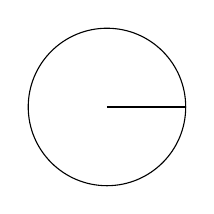
\begin{tikzpicture}
	\draw (0, 0) circle (1cm);
	\draw (0, 0) -- (1,0);
\end{tikzpicture}

To express every complex number $w^n = z$ we end up with the following generalization:
\begin{defn}[\textbf{Root of Unity}]
	\[\zeta^k = e^{\sfrac{2\pi ik}{n}}\]
\end{defn}
Which has the $n$th power given as:
\[ (\zeta^k)^n = ( e^{\sfrac{2\pi ik}{n}} )^n = e^{2\pi ik} = 1 \]
The points $w_k$ are just the product of $e^{\frac{i\theta}{n}}$ with all the $n$-th roots of unity:
\[w_k = e^{\sfrac{i\theta}{n}}\zeta^k\]
\\
One of the \textbf{major results of the theory of complex variables} is to reduce the study of certain functions, including most of the common functions we know like exponentials, logarithms, sine, cosine; to power series, which can be approximated by polynomials.\\

Thus the power function is in some sense the unique basic function out of which the others are constructed.


\subsection{Proofs}
\begin{enumerate}
	\item Let $f(z) = \sfrac{1}{z}.$ Describe what $f$ does to the inside and ouside of the unit circle, and also, what it does to points on the uit circle. This map is called \textbf{inversion} through the unit circle. \\
	
	\textbf{Proof:} \\
	Take the points $|z| < 1$ and move them to outside the unit disc.
	\begin{align*}
		&z < 1 \\
		&z \mapsto \frac{1}{z} > 1
	\end{align*}
	\\
	Then, Take the points outside the unit circle $|z| > 1$ and put them in the unit circle:
	\begin{align*}
		&z > 1 \\
		&z \mapsto \frac{1}{z} < 1
	\end{align*}
	\qed


	\item Let $f(z) = \sfrac{1}{\bar{z}}.$ Describe $f$ in the same manner as Exercise 1. 
	This map is called \textbf{reflection} through the unit circele. \\
	
	\textbf{Proof:} \\
	Take a point outside the unit circle, $|z| > 1$, reflect it across the line of symmetry to $\bar{z}$ and then map it to the same quadrant inside the unit circle:
	\begin{align*}
		z \mapsto \sfrac{1}{\bar{z}} \\
	\end{align*}

	Take a point inside the unit circle, $0 < |z| < 1$, reflect it across the line of symmetry to $\bar{z}$ and then map it to the same quadrant outside the unit circle. 
	\qed


	\item Let $f(z) = e^{2\pi iz}.$ Describe the image under $f$ of the set consisting of the points $x + iy$ with:
	\[ \frac{-1}{2} \leq x \leq \frac{1}{2} \]
	and
	\[ y \geq B := \{ z = x + iy \;\;|\;\; y > 0 \} \] \\

	\textbf{Proof:} \\

	\item Let $f(z) = e^z.$ Describe th image under $f$ of the following sets:
	\begin{enumerate}
		\item The set of $z = x + iy$ such that $x \leq 1$ and $0 \leq y \leq \pi.$ \\
		
		\textbf{Proof:} \\

		\item The set of $z = x + iy$ such that $0 \leq y \leq \pi$ and no condition on $x.$ \\
		
		\textbf{Proof:} \\

	\end{enumerate}
	
\end{enumerate}

\subsection{Incomplete Proofs}
\begin{itemize}
	\item 3, 4
\end{itemize}


\section{Limits and Compact Sets}
\subsection{Limits In $\mathbb{C}$}

\begin{defn}[\textbf{Open Disc of radius $r > 0$ centered at $\alpha$}]
	The set $S \subset \mathbb{C}$ with elements $z$ such that:
	\[ |z - \alpha | < r \]
	Denoted $D(\alpha, r).$
\end{defn}

\begin{defn}[\textbf{Open Set $U \subset \mathbb{C}$}]
	$U$ is an open set if for every point $\alpha \in U$:
	\begin{enumerate}
		\item there is a disc $D(\alpha,r)$ centered at $\alpha$
		\item there is a disc of some radius $r > 0$ such that this disc $D(\alpha, r)$ is contained in $U.$
	\end{enumerate}
\end{defn}

\begin{defn}[\textbf{Boundary Point of $S$}]
	A point $\alpha$ such that every disc $D(\alpha, r)$ centered at $\alpha$ and of 
	radius $r > 0$ contains both points of $S$ and points not in $S.$
\end{defn}

\begin{defn}[\textbf{Adherent Point to $S$}]
	$\alpha$ is adherent to $S$ if: 
	\begin{itemize}
		\item every disc $D(\alpha, r)$ with $r > 0$ contains \textit{some} element of $S.$
	\end{itemize}
\end{defn}

\begin{defn}[\textbf{Interior point to $S$}]
	$\alpha$ is an interior point of $S$ if:
	\begin{itemize}
		\item there exists a disc $D(\alpha, r)$ which is contained in $S.$
	\end{itemize}
\end{defn}

Note that:
\begin{itemize}
	\item An adherent point can be a boundary point
	\item An adherent point can be an interior point
\end{itemize}

\begin{defn}[\textbf{Closed Set}]
	A set is closed if it contains all its boundary points.
\end{defn}

\begin{defn}[\textbf{Bounded Set}]
	$S$ is bounded if there exists a number $C > 0$ such that:
	\begin{align*}
		|z| \leq C \;\;\;\;\; \forall z \in S
	\end{align*}
\end{defn}

\begin{defn}[\textbf{Closure of a Set $S$}]
	The unioin of $S$ and all its boundary points.
	\begin{itemize}
		\item Denoted $\bar{S}$
	\end{itemize}
\end{defn}

\begin{defn}[\textbf{Limit of $f$}]
	
\end{defn}
\begin{itemize}
	\item Let $f$ be a function on $S \subseteq \mathbb{C}.$ 
	\item Let $\alpha$ be an adherent point of $S.$ 
	\item Let $w$ be a complex number. 
\end{itemize}
We say that:
	\[ z \in S \]
	\[ \lim_{z \to \alpha} f(z) = w \]
If given $\epsilon > 0$ there exists $\delta > 0$ such that if $z \in S$ and $|z - \alpha| < \delta,$ then:
\[ |f(z) - w | < \epsilon \]

\begin{defn}[\textbf{Continuous}]
	$f$ is continuous at $\alpha$ if:
	\[ \lim_{z \to \alpha} f(z) = f(\alpha) \]
\end{defn} 

\begin{defn}[\textbf{Cauchy Sequence}]
	If $\epsilon > 0$ then $\exists \; N$ such that if:
	\[ m, n \geq N \]
	then:
	\[| \; {z}_{n} - {z}_{m} \; | < \epsilon \]
\end{defn}

\subsection{Compact Sets}
This section is a bit peculiar and full of theorems I've not had a use for yet, but may be useful later. The main point is this:
\begin{thm}
	A set $S$ is compact $\iff$ it is closed and bounded.
\end{thm}

\subsection{Sequence of Complex Numbers: my note}

\begin{defn}[\textbf{Sequence of Complex Numbers}]
	A function defined on the set of Natural numbers whose 
	range is contained in the set of Complex numbers.
	\[n \to z\]
\end{defn}

If a sequence has a limit, it converges. Else, it diverges.

\subsection{Proofs}
\begin{enumerate}
	\item 
	\subitem a. Let $\alpha$ be a complex number of absolute value $< 1.$ 
	What is $\lim\limits_{n \to \infty} \alpha^n ?$ Proof?

	\textbf{Proof:} \\
	Just use a Cauchy Sequence.

	$|\alpha| < 1$ iff $ |\alpha| = \frac{1}{|z|}.$ 

	So then check $\lim\limits_{n \to \infty} |\alpha|^n$:
	\begin{align*}
		\lim\limits_{n \to \infty} |\alpha|^n &= \lim\limits_{n \to \infty} \frac{1}{|z|^n} \\
	\end{align*}
	This sequence has different behavior for $z < 1$ vs $z > 1$, but we must have $|\alpha| < 1$ therefore $z > 1$ only here.

	\begin{align*}
		\lim\limits_{n \to \infty} |\alpha|^n &= \lim\limits_{n \to \infty} \frac{1}{|z|^n} \\
	\end{align*}

	Since $z > 1$ and by the Archimedean principal we can always find $m > n$
	then clearly: 
	\begin{align*}
	\alpha^m < \alpha^n \iff \frac{1}{z^m} < \frac{1}{z^n}
	\end{align*}
	
	Therefore this sequence is monotonic, it only decreases each new term, and the difference between $m, n$ terms is 
	small but always $> 0$ which gives us a cauchy sequence.

	So then:
	\begin{align*}
		|\alpha^n - \alpha^m| < \epsilon \\
	\end{align*} \qed
	\\
	\subitem b. Let $\alpha$ be a complex number of absolute value $> 1.$ 
	What is $\lim\limits_{n \to \infty} \alpha^n ?$ Proof?

	\textbf{Proof:} \\
	$ \alpha = |z| > 1$ and $\alpha_n = |z|^n.$ 
	Looking at the \textit{limit of the sequence} we see it increasing arbitrarily, and so each 
	term is larger than the previous which means we can't ever satisfy our definition of a limit 
	since we \textit{can} choose some $m, n$ that would have some arbitrarily large difference between 
	them $> \epsilon.$ \qed
	
	\item Show that for any complex number $z \neq 1,$ we have
	\[ 1 + z + \cdots + z^n = \frac{z^{n + 1} - 1}{z - 1}\]
	If $|z| < 1,$ show that
	\[ \lim_{n \to \infty} (1 + z + \cdots + z^n ) = \frac{1}{1 - z} \] \\
		
	\textbf{Proof:} \\
	Now we need to look at the \textit{limit of a sequence of partial sums} and test convergence. \\

	\begin{align*}
		S_1 &= 1 \\
		S_2 &= 1 + z \\
		S_3 &= 1 + z + z^2 \\
		\vdots &= \vdots \\
		S_n &= 1 + z + z^2 + \cdots + z^n
	\end{align*}
	Now play with the algebra and multiply both sides by $z$ for shits and giggles
	\begin{align*}
		zS_n &= z + z^2 + \cdots + z^{n +1} \\
		zS_n - S_n &= z + z^2 + \cdots + z^{n +1} - S_n \\
		S_n(z - 1) &= z + z^2 + \cdots + z^{n +1} - S_n \\
	\end{align*}
	The telescoping series starts to look more obvious
	\begin{align*}
		S_n(z - 1) &= z + z^2 + \cdots + z^{n +1} - (1 + z + z^2 + \cdots + z^n) \\
	\end{align*}
	Matching up the pairs we see the result we need
	\begin{align*}
		S_n(z - 1) &= z + z^2 + \cdots + z^{n +1} - 1 - z - z^2 - \cdots - z^n) \\
		S_n(z - 1) &= z^{n +1} - 1 + z - z + z^2 - z^2 + z^3 - z^3 + \cdots + z^n - z^n) \\
		\therefore S_n &= \frac{z^{n +1} - 1}{z - 1} \\
	\end{align*}
	And now we do as we said, \textit{take the limit of a sequence of partial sums}
	\begin{align*}
		\lim_{n \to \infty} S_n &= \lim_{n \to \infty} \frac{z^{n +1} - 1}{z - 1} \\
	\end{align*}
	And clearly this sequence diverges if $|z| > 1$ since the numerator grows unbounded over a fixed denominator. \\

	Now consider if $|z| < 1$ and 
	\begin{align*}
		\lim_{n \to \infty} S_n &= \lim_{n \to \infty} \frac{z^{n +1} - 1}{z - 1} \\
		&=  \frac{- 1}{z - 1} \\
		&=  \frac{1}{1 - z} \\
		\therefore \lim_{n \to \infty} (1 + z + \cdots + z^n ) &= \frac{1}{1 - z}
	\end{align*}
	\qed

	\item Let $f$ be the function defined by
	\[ f(z) = \lim_{n \to \infty} \frac{1}{1 + n^2 z} \]
	Show that $f$ is the characteristic function of the set $\{0\},$ that is, $f(0) = 1,$ and $f(z) = 0$ if $z \neq 0.$ \\
			
	\textbf{Proof:} \\

	\item For $|z| \neq 1$ show that the following limit exists:
	\[ f(z) = \lim_{n \to \infty} \left( \frac{z^n - 1}{z^n + 1} \right) \]

	Is it possible to define $f(z)$ when $|z| = 1$ in such a way to make $f$ continuous? \\
		
	\textbf{Proof:} \\


	\item Let
	\[ f(z) = \lim_{n \to \infty} \frac{z^n}{1 + z^n} \]
	\begin{enumerate}
		\item What is the domain of definition of $f,$ that is, for which complex numbers $z$ does the limit exist? \\
		
		\textbf{Proof:} \\
	
		\item Give explicitly the values of $f(z)$ for the various $z$ in the domain of $f.$

		\textbf{Proof:}
	
	\end{enumerate}

	\item Show that the series
	\[ \sum_{n = 1}^{\infty} \frac{z^{n - 1}}{(1 - z^n )(1 - z^{n + 1})} \]
	Converges to
	\[ \frac{1}{(1 - z)^2 } \;\;\; |z| < 1 \]
	and
	\[\frac{1}{z(1 - z)^2 } \;\;\; |z| > 1\]

	Prove that the convergence is uniform for $|z| \leq c < 1$ in the first case, and $|z| \geq b > 1$ in the second case. 

	[\textit{Hint:} multiply and divide each term by $1 - z,$ and do a partial fraction decomposition, getting a telescoping effect. ]

	\textbf{Proof:}
	
	For this problem, just follow along with Lang's suggestion and watch the telescope emerge. Let's look at the $n$th term for $z$ and see 
	if there's something there.

	\begin{align*}
		z_n &= \frac{z^{n - 1}}{(1 - z^{n})(1 - z^{n + 1})} \\
		z_n \cdot \frac{(1 - z)}{(1 - z)} &= \frac{z^{n - 1}}{(1 - z^{n})(1 - z^{n + 1})} \\
		z_n (1 - z) &= (1 - z) \cdot \frac{z^{n - 1}}{(1 - z^{n})(1 - z^{n + 1})} \\
		z_n (1 - z) &=  \frac{(1 - z)z^{n - 1}}{(1 - z^{n})(1 - z^{n + 1})} \\
		z_n (1 - z) &=  \frac{z^{n - 1} - z^n}{(1 - z^{n})(1 - z^{n + 1})} \\
	\end{align*}

	Now use a \textbf{partial fraction decomposotion} here:

	\begin{align*}
		\frac{z^{n - 1} - z^n}{(1 - z^{n})(1 - z^{n + 1})} &=  \frac{z^{n - 1}}{(1 - z^{n})} - \frac{z^n}{(1 - z^{n + 1})} \\
	\end{align*}

	So then

	\begin{align*}
		z_n (1 - z) &=  \frac{z^{n - 1}}{(1 - z^{n})} - \frac{z^n}{(1 - z^{n + 1})} \\
		\therefore \;\;\; z_n &=  \frac{1}{(1 - z)} \left( \frac{z^{n - 1}}{1 - z^{n}} - \frac{z^n}{1 - z^{n + 1}} \right) \\
	\end{align*}

	And then we see the terms create telescoping terms between them using this new expression

	\begin{align*}
		z_1 &= \frac{1}{(1 - z)} \left( \frac{z^{1 - 1}}{1 - z^{1}} - \frac{z^1}{1 - z^{1 + 1}} \right) \\
		&= \frac{1}{(1 - z)} \left( \frac{1}{1 - z} - \frac{z}{1 - z^{2}} \right) \\
		&= \frac{1}{(1 - z)^2} - \frac{z}{(1 - z)(1 - z^{2})} \\
	\end{align*}

	And then note

	\begin{align*}
		z_2 &= \frac{1}{(1 - z)} \left( \frac{z^{2 - 1}}{1 - z^{2}} - \frac{z^2}{1 - z^{2 + 1}} \right) \\
		&= \frac{1}{(1 - z)} \left( \frac{z}{1 - z^2} - \frac{z^2}{1 - z^{3}} \right) \\
		&= \frac{z}{(1 - z)(1 - z)^2} - \frac{z}{(1 - z)(1 - z^{2})} \\
	\end{align*}

	And so 

	\begin{align*}
		z_1 + z_2 &= \frac{1}{(1 - z)^2} - \frac{z}{(1 - z)(1 - z^{2})} + \frac{z}{(1 - z)(1 - z)^2} - \frac{z}{(1 - z)(1 - z^{2})} \\
		z_1 + z_2 &= \frac{1}{(1 - z)^2} - \frac{z}{(1 - z)(1 - z^{2})} \\
	\end{align*}

	And so now we see how the terms will match up and we are left with

	\begin{align*}
		z_1 + z_2 + \cdots + z_n &= \frac{1}{(1 - z)^2} \\
		&- \frac{z}{(1 - z)(1 - z^{2})} + \frac{z}{(1 - z)(1 - z)^2} \\
		&- \frac{z^2}{(1 - z)(1 - z^{2})} + \frac{z^2}{(1 - z)(1 - z^{2})} + \cdots \\
		&- \frac{z^n-1}{(1 - z)(1 - z^{n})} +\frac{z^n-1}{(1 - z)(1 - z^{n})} - \frac{z^n}{(1 - z)(1 - z^{n + 1})} \\
		&= \frac{1}{(1 - z)^2} - \frac{z^n}{(1 - z)(1 - z^{n + 1})} \\
	\end{align*}

	And so clearly for the case $|z| < 1$ and taking the $\lim n \to \infty$ the last term goes to $0$ and we are left with the desired result.
\end{enumerate}

\subsection{Incomplete proofs}
4, 5, 6

\section{Complex Differentiability}
\textit{(There are no exercises in this section.)}
\begin{itemize}
	\item Let $U$ be an open set. 
	\item Let $f$ be a function on $U.$
\end{itemize}

\begin{defn}[$f$ \textbf{Complex Differentiable at} $z$]
	If the limit exists:
	\begin{align*}
		\lim_{h \to 0} \frac{f(z + h) - f(z)}{h} \\
	\end{align*}


	denoted by $f'(z)$ or $df/dz.$
\end{defn}
\begin{itemize}
	\item \textit{Note:} If $f$ is differentiablre at $z$ then $f$ is continuous at $z.$
\end{itemize}

All that really matters in this section 
is that all the usual rules for sums, products, quotients, and functions of functions are the same 
wrt complex Differentiability as they were with real Differentiability.

\subsection{Holomorphic Function}
A function $f$ defined on an open set $U$ is said to be \textbf{differentiable} if it is differentiable at every point.
\begin{itemize}
	\item Also say that $f$ is \textbf{Holomorphic} on $U.$
	\item Holomorphic is usually used to specify \textit{complex} differentiability as distinguised from \textit{real} differentiability.
\end{itemize}


\begin{defn}[\textbf{Holomorphic Isomorphism}]
	A holomorphic function
	\begin{align*}
		f: U \to V
	\end{align*}
	From an open set into another open set is a \textbf{holomorphic isomorphism} if there exists a holomorphic function
	\begin{align*}
		g: V \to U
	\end{align*}
	such that $g$ is the inverse of $f.$ That is;
	\begin{align*}
		g \circ f &= id_u \,\,\,\,
		and \,\,\,\,
		f \circ g = id_v
	\end{align*}
\end{defn}

\begin{defn}[\textbf{Holomorphic Automorphism}]
	A holomorphic isomorphism of an open set $U$ with itself.
\end{defn}

\section{The Cauchy-Reimann Equations}
In this section:
\begin{itemize}
	\item Let $f$ be a function on an open set $U.$
	\item Write $f$ in terms of its \textit{real} and \textit{imaginary} parts.
	\begin{align*}
		f(x + iy) = u(x, y) + iv(x, y) \\
	\end{align*}
	\item We derive the equivalent conditions on $u$ and $v$ for $f$ to be holomorphic.
\end{itemize}

At a fixed $z$: 
\begin{itemize}
	\item let $f'(z) = a + bi.$ \\
	\item let $w = h + ik \,\,\,\, h, k \in \mathbb{R}$
	\item Suppose:
	\begin{align*}
		\lim_{w \to 0} \sigma(w) &= 0 \\
		f(z + w) - f(z) &= f'(z)w + \sigma(w)w \\
	\end{align*}
	\item Let:
	\begin{align*}
		\vec{F}: U \to \mathbb{R}^2 \\
	\end{align*}
	\item such that:
	\begin{align*}
		\vec{F}(x, y) &= (u(x, y), v(x, y))
	\end{align*}
\end{itemize}

\begin{itemize}
		\item We call $\vec{F}$ the (real) \textbf{Field Associated with} $f.$ 
		\item If we assume that $f$ is holomorphic then $\vec{F}$ is differentiable, and its derivative is represented by the \textbf{Jacobian Matrix}:
		\begin{align*}
			J_{\vec{F}}(x, y) = \left( \begin{matrix}
				a & -b \\
				b &\,\,\,\,  a 
			\end{matrix}
			\right)
			= \left( \begin{matrix}
				\frac{\partial u}{\partial x} & \frac{\partial u}{\partial y} \\
				\frac{\partial v}{\partial x} & \frac{\partial v}{\partial y}
			\end{matrix} \right)
		\end{align*}
		\item This shows:
		\begin{align*}
			f'(z) = \frac{\partial u}{\partial x} - i\frac{\partial u}{\partial y}
		\end{align*}
\end{itemize}
This all culminates to the incredibly important result of:
\begin{defn}[\textbf{Cauchy-Riemann Equations}]
	\begin{align*}
		\frac{\partial u}{\partial x} = \frac{\partial v}{\partial y} \,\,\,\, \text{and} \,\,\,\, \frac{\partial u}{\partial y} = -\frac{\partial v}{\partial x}
	\end{align*}	
\end{defn}


Last bit over Jacobian Determinant $\triangle_{\vec{F}}$ needed.

\subsection{Proofs}
\begin{enumerate}
	\item Prove in detail that if $u, v$ satisfy the Cauch-Riemann equations, then the function
	\begin{align*}
		f(z) = f(x + iy) = u(x, y) + iv(x, y) \\
	\end{align*}
	is holomorphic.
\end{enumerate}
\begin{proof}
	Let $u,v$ satisfy the Cauchy-Riemann equations.
\end{proof}

\section{Angles Under Holomorphic Maps}
\textit{(There are no exercises in this section.)}

What is important here is a simple geometric property of holomorphic maps. Roughly speaking, they preserve angles.

